\documentclass{beamer}
\usepackage{pgfpages}
%\setbeameroption{show notes on second screen=left} %enable for notes
\usepackage{graphicx}
\usepackage{xcolor}
\usepackage{listings}
%\usepackage{transparent}
\usepackage{hyperref}
\lstset{language=python,frame=single}
\usepackage{verbatim}
%\usepackage{apacite}
\usepackage[longnamesfirst]{natbib}
\usepackage{subcaption}
\usepackage{amsmath}
\usepackage{relsize}
\usepackage{appendixnumberbeamer}
\usepackage{xparse}
\usepackage{multimedia}
\usepackage{xcolor}
\usepackage[normalem]{ulem}
\usepackage{tikz}
\usetikzlibrary{matrix,backgrounds}
\usetikzlibrary{positioning}
\usetikzlibrary{shapes,arrows}
\usetikzlibrary{positioning}

\tikzset{onslide/.code args={<#1>#2}{%
  \only<#1>{\pgfkeysalso{#2}} 
}}

\tikzstyle{block} = [rectangle, draw, fill=red!20!blue!10, 
    text width=5em, text centered, rounded corners, minimum height=4em]
\tikzstyle{netnode} = [circle, draw, very thick, inner sep=0pt, minimum size=0.5cm] 
\tikzstyle{relunode} = [rectangle, draw, very thick, inner sep=0pt, minimum size=0.5cm] 
    
\tikzstyle{line} = [draw, line width=1.5pt, -latex']

\pgfdeclarelayer{background}
\pgfsetlayers{background,main}

\pgfdeclarelayer{myback}
\pgfsetlayers{myback,background,main}

\usetheme[numbering=fraction]{metropolis}
\newcommand{\semitransp}[2][35]{\color{fg!#1}#2}

\newcommand\blfootnote[1]{%
  \begingroup
  \renewcommand\thefootnote{}\footnote{#1}%
  \addtocounter{footnote}{-1}%
  \endgroup
}
\renewcommand*\footnoterule{}
%%\AtBeginSection[]
%%{
%%  \begin{frame}
%%    \frametitle{Table of Contents}
%%    \tableofcontents[currentsection]
%%  \end{frame}
%%}

\begin{document}

\title{Multi-task learning \& generalization}
\author{Andrew Lampinen}
\date{}
\frame{\titlepage}

\begin{frame}[standout]
Connectionist modeling has too often focused on single tasks.\par
\end{frame}

\begin{frame}[fragile]{Multi-task learning in ML}
\uncover<2->{
\begin{figure}
\centering
\begin{tikzpicture}[remember picture, overlay, every node/.style={inner sep=0,outer sep=0}]
\node [anchor=center, draw, fill=white, minimum width=2cm, minimum height= 1 cm] at (current page.center) (brain) {\Large RNN};
\only<-4>{
\node [anchor=center, below left = 1cm and 0.25cm of brain] (input1) {``Ceci n'est pas une pipe.''};
\node [anchor=center, above left = 1cm and 0.25cm of brain] (output1) {``This is not a pipe.''};
}

\only<-4>{
\node<3-4> [anchor=center, below right = 0.45cm and 0.25cm of brain] (input2) {\includegraphics[width=0.25\textwidth]{figures/un_pipe.jpg}};
\node<3-4> [anchor=center, above right = 1cm and 0.25cm of brain] (output2) {``This is a pipe.''};
}

\only<5->{
\node [anchor=center, below left = 1.25cm and 1cm of brain] (mi1) {French};
\node [anchor=center, above left = 1.25cm and 1cm of brain] (mo1) {Chinese};
\node [anchor=center, below left = 2cm and -0.25cm of brain] (mi2) {Swahili};
\node [anchor=center, above left = 2cm and -0.25cm of brain] (mo2) {German};

\node [anchor=center, below right = 1.25cm and 1cm of brain] (mi4) {English};
\node [anchor=center, above right = 1.25cm and 1cm of brain] (mo4) {Italian};
\node [anchor=center, below right = 2cm and -0.25cm of brain] (mi3) {Spanish};
\node [anchor=center, above right = 2cm and -0.25cm of brain] (mo3) {Korean};
}

\begin{pgfonlayer}{background}
\only<-4>{
\path [line] (input1.east) to [out=45, in=-45] (output1.east);
\path<3-4> [line] (input2.west) to [out=135, in=-135] (output2.west);
}
\only<5->{
\path [line] (mi1.east) to [out=10, in=-10] (mo1.east);
\path [line] (mi2.north east) to [out=70, in=-70] (mo2.south east);
\path [line] (mi4.west) to [out=170, in=-170] (mo4.west);
\path [line] (mi3.north west) to [out=110, in=-110] (mo3.south west);
}
\end{pgfonlayer}
\only<4>{
\path [line, line width=3 pt, red, dashed] ([xshift=0.44cm]input1.north) to node [anchor=center, text width=2.5cm, align=center, xshift=-1.5cm] {Better generalization!} (output1.south);
}
\only<6->{
\path [line, line width=3 pt, red, dashed] (mi4.west) to node [anchor=center, xshift=3cm] {No training needed!} (mo1.east);
}
\end{tikzpicture}
\end{figure}
\vspace{2em}
\blfootnote{\uncover<4->{
    \only<i
    \only<1,5->{\citep{Johnson2016a}}
}}
}
\end{frame}

\begin{frame}[standout]
Multi-task learning can substantially improve generalization in neural networks.\par
\end{frame}

\begin{frame}{Humans face many related tasks}
\begin{figure}
\centering
\begin{subfigure}{0.4\textwidth}
\includegraphics[width=\textwidth]{figures/chess_cropped.jpg}
\end{subfigure}%
\begin{subfigure}{0.4\textwidth}
\includegraphics[width=\textwidth]{figures/go2.jpg}
\end{subfigure}\\
\uncover<2>{
\begin{subfigure}{0.4\textwidth}
\includegraphics[width=\textwidth]{figures/math.jpg}
\end{subfigure}%
\begin{subfigure}{0.4\textwidth}
\includegraphics[width=\textwidth]{figures/piano.jpg}
\end{subfigure}%
}
\end{figure}
\uncover<2->{
\scriptsize
\only<1>{\vspace{-1.3em}}
\citep{Lampinen2017a, Hansen2017}
}
\note{There are deep relationships among the tasks we do -- some are superficially obvious, like Go and Chess, and some are less so, like the mathematical structures underlying music or the fact that we use language to talk about all these domains.}
\end{frame}

\begin{frame}{Multi-task learning is also beneficial on smaller scales}
\begin{figure}
\vspace{2em}
\centering
\begin{subfigure}{0.3\textwidth}
\includegraphics[width=\textwidth]{figures/hexagon_arrow.png}
\end{subfigure}~
\begin{subfigure}{0.65\textwidth}
\includegraphics[width=\textwidth]{figures/fyp_1_modular_text.png}
\end{subfigure}
\vspace{2em}
\end{figure}
{
\scriptsize
\citep{Lampinen2017b}
}
\end{frame}

\begin{frame}[standout]
Our models should reflect the fact that human intelligence is multi-purpose.\par
\end{frame}

\begin{frame}{Multi-task benefits (and costs)}
\begin{figure}
\centering
\only<1>{
\vspace{3em}
\includegraphics[width=\textwidth]{figures/analytic_paper_title.png}
}
\only<2>{
\vspace{3em}
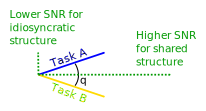
\includegraphics[width=0.8\textwidth]{figures/transfer_pros_cons.png}
\vspace{1.25em}
}
\only<3>{
\vspace{2em}
\begin{subfigure}{0.3\textwidth}
\includegraphics[width=\textwidth]{figures/fig_5a.png}
\end{subfigure}~
\begin{subfigure}{0.3\textwidth}
\includegraphics[width=\textwidth]{figures/transfer_by_alignment.png}
\end{subfigure}~
\begin{subfigure}{0.4\textwidth}
\includegraphics[width=\textwidth]{figures/fig_5c.png}
\end{subfigure}
%%\includegraphics[width=0.5\textwidth]{figures/transfer_by_alignment.png}
}
\end{figure}
\vspace{1em}
\blfootnote{\uncover<2->{\citep*{Lampinen2018}}}
\end{frame}


\begin{frame}[standout]
When the target task is noisy or auxiliary tasks are well aligned, transfer is very beneficial.
\end{frame}

\begin{frame}[fragile]{Limitations of deep learning, or of tasks?}
\begin{figure}
\vspace{-2em}
\centering
\begin{tikzpicture}[remember picture, overlay, every node/.style={inner sep=0,outer sep=0}]
\node [anchor=center, align=center,] at (-1, 0) (c0) {\includegraphics[width=7cm]{figures/critique0.png}};
\node [anchor=center, align=center,] at (0, 0) (c1) {\includegraphics[width=7cm]{figures/critique1.png}};
\node [anchor=center, align=center,] at (1, -2) (c2) {\includegraphics[width=7cm]{figures/critique2.png}};
\end{tikzpicture}
\end{figure}
\vspace{2em}
\end{frame}

\begin{frame}[standout]
Data-hunger and failures to generalize may be due to ``poverty of the [training] stimulus'' -- humans do many more tasks than our models.\par
\end{frame}

%%\begin{frame}[fragile]{Meta-learning in ML}
%%\begin{figure}
%%\centering
%%\begin{tikzpicture}[remember picture, overlay, every node/.style={inner sep=0,outer sep=0}]
%%\node [anchor=center, draw, fill=white, minimum width=3cm, minimum height= 1 cm] at ([yshift=-2cm]current page.center) (brain) {\Large RL network};
%%\node [anchor=center, above = 1cm of brain] (output1) {
%%\only<1>{\includegraphics[height=3.5cm]{figures/slot_machine.jpeg}}
%%\only<2>{\includegraphics[height=4cm]{figures/casino.jpg}}
%%};
%%
%%\path [line] (brain.north) to (output1.south);
%%\end{tikzpicture}
%%\end{figure}
%%\vspace{1em}
%%\blfootnote{\uncover<2->{\citep{Duan2016, Wang2016a}}}
%%\end{frame}
%%
%%\begin{frame}{Humans face many related tasks (again)}
%%\begin{figure}
%%\centering
%%\begin{subfigure}{0.4\textwidth}
%%\includegraphics[width=\textwidth]{figures/chess_cropped.jpg}
%%\end{subfigure}%
%%\begin{subfigure}{0.4\textwidth}
%%\includegraphics[width=\textwidth]{figures/go2.jpg}
%%\end{subfigure}
%%\end{figure}
%%\uncover<2->{
%%\begin{exampleblock}{}
%%Meta learning matches the perspective of educational researchers who describe education as ``Preparation for Future Learning'' \citep{Bransford1999}.
%%\end{exampleblock}
%%}
%%\note{There are deep relationships among the tasks we do -- some are superficially obvious, like Go and Chess, and some are less so, like the mathematical structures underlying music or the fact that we use language to talk about all these domains.}
%%\end{frame}





%%
%%\begin{frame}{Background}
%%\begin{itemize}
%%\item Not a new idea: transfer has been called a central component of ``why we're so smart'' \citep{Gentner2003}, and an important source of new ideas \citep{Gick1980}.
%%\item<2->
%%However, this perspective has been criticized!\par
%%\begin{itemize}
%%\item<3-> ``Significant transfer is probably rare and accounts for very little human behavior. ... We generally do what we have learned to do and no more.'' \citep{Detterman1993}
%%\end{itemize}
%%\item<4-> How can we reconcile these different viewpoints?
%%\end{itemize}
%%\note{Detterman: ``We generally do what we have learned to do and no more.'' Experimental manipulations in transfer experiments ``have the subtlety of a baseball bat.''\par
%%Observation from FriSem last year: there is a correlation between the speed of transfer being sought and how important they think it is.}
%%\end{frame}
%%
%%\begin{frame}{Transfer speed}
%%\vspace{1.5em}
%%I think there's a neglected variable: speed of transfer.\par
%%\uncover<2->{
%%\begin{center}
%%\begin{table}
%%\begin{tabular}{|c|c|}
%%\hline
%%Fast & Slow \\
%%\hline
%%\parbox{0.45\textwidth}{
%%    \begin{itemize}
%%    \item<2-> one (or a few) examples explicitly shown
%%    \item<3-> transfer requires explicit awareness of analogy
%%    \end{itemize}
%%}
%%&
%%\parbox{0.45\textwidth}{
%%    \begin{itemize}
%%    \item<2-> learning gradually through many interactions
%%    \item<3-> {transfer may or may not be explicit}%
%%               %%\only<4>{\color{red}transfer may or may not be explicit}}
%%    \end{itemize}
%%}\\ \hline
%%\end{tabular}
%%\end{table}
%%}
%%\vspace{1.5em}
%%\note{E.g. being told about the rules of chess and then seeing if that helps you play go, vs. playing many games of chess and go and seeing if one helps the other}
%%\end{center}
%%{
%%\scriptsize
%%\citep{Lampinen2017a}
%%}
%%\end{frame}
%%
%%\begin{frame}{Transfer speed and outcomes}
%%For example, imagine you are about to teach someone to play guitar. Who do you think would likely perform better:
%%\begin{itemize}
%%\item a person who has just taken their first piano lesson 
%%\item a person who has been playing piano for years
%%\end{itemize}
%%\begin{figure}
%%\centering
%%\begin{subfigure}{0.4\textwidth}
%%\includegraphics[width=\textwidth]{figures/piano.jpg}
%%\end{subfigure}~%
%%\begin{subfigure}{0.4\textwidth}
%%\includegraphics[width=\textwidth]{figures/guitar.jpg}
%%\end{subfigure}%
%%\end{figure}
%%\note{So transfer may require slow learning in the original domain to set up sufficiently high-quality representations to see an effect}
%%\end{frame}
%%
%%\begin{frame}{Transfer speed and opinions}
%%Transfer speed helps reconcile why some people think transfer is important, while others don't. 
%%\begin{figure}
%%\centering
%%\includegraphics[width=0.5\textwidth]{figures/perspectives_on_transfer.png}
%%\end{figure}
%%\end{frame}
%%
%%
%%\begin{frame}[standout]
%%Slow transfer between tasks is important.
%%\end{frame}
%%
%%\begin{frame}{Abstraction and transfer}
%%We often progress from procedural to more explicit, abstract, or formal knowledge: \vspace{-0.2em}
%%\begin{figure}
%%\centering
%%\begin{tikzpicture}
%%\node (img1) {\includegraphics[width=0.33\textwidth]{figures/multiplication_procedural_smaller.png}};
%%\uncover<2->{
%%\node (img2) at ([yshift=-2em]img1.east) {\includegraphics[width=0.33\textwidth]{figures/factoring_polynomial_worksheet.png}};
%%}
%%\uncover<3->{
%%\node (img3) at ([yshift=-3em]img2.east) {\includegraphics[width=0.5\textwidth]{figures/prime_ideals.png}};
%%}
%%\end{tikzpicture}
%%\end{figure}\vspace{-0.2em}
%%\uncover<4>{These are related tasks that share some structure! Is it useful to think about this from the perspective of transfer?}
%%\note{worksheetfun.com\par
%%Less abstract and more abstract reasoning can be seen as partially distinct tasks that share some common structure. There are different ways that procedural knowledge could support more formal, setting up representations and intuitions, having examples to reason over, ...}
%%\end{frame}
%%
%%\begin{frame}{Is abstraction transfer?}
%%Yet there are also times when procedural and formal knowledge seem partially dissociable:
%%\begin{figure}
%%\centering
%%\begin{subfigure}{0.4\textwidth}
%%\includegraphics[width=\textwidth]{figures/piano.jpg}
%%\end{subfigure}~%
%%\begin{subfigure}{0.5\textwidth}
%%\includegraphics[width=\textwidth]{figures/mixolydian.png}
%%\end{subfigure}%
%%\end{figure}
%%\note{}
%%\end{frame}
%%
%%\begin{frame}[standout]
%%When and how do procedural and more explicit, abstract, or formal knowledge influence each other?
%%\end{frame}
%%
%%\begin{frame}<-8>[label=phenomena]
%%\frametitle<-9>{A diagram of potential phenomena of interest}
%%\frametitle<10>{What explicit knowledge?}
%%\vspace{-1em}
%%\begin{figure}
%%\centering
%%\begin{tikzpicture}[auto] %% TODO? highlighting
%%\node [rectangle, draw, thick, text width=2cm, align=center, onslide={<10>,{opacity=0.2}}] (A) at (-4, 0) {Task A}; 
%%\node [rectangle, draw, thick, text width=2cm, align=center, onslide={<10>,{opacity=0.2}}] (B) at (4, 0) {Task B}; 
%%\path [line, dashed, <->, onslide={<10>,{opacity=0.2}}] (A.east) to node[text width=2cm] (underlying) {Underlying relationship} (B.west); 
%%
%%\uncover<2->{
%%\node [rectangle, draw, thick, text width=2cm, align=center, onslide={<10>,{opacity=0.2}}] (Aproc) at (-4, 2) {Ability to perform  A}; 
%%\node [rectangle, draw, thick, text width=2cm, align=center, onslide={<10>,{opacity=0.2}}] (Bproc) at (4, 2) {Ability to perform B}; 
%%\path [line, ->, dashed, onslide={<10>,{opacity=0.2}}] (A.north) to  node (Atrans) {}(Aproc.south); 
%%\path [line, ->, dashed, onslide={<10>,{opacity=0.2}}] (B.north) to node (Btrans) {} (Bproc.south); 
%%}
%%
%%\uncover<3->{
%%\path [line, ->, onslide={<10>,{opacity=0.2}}] (Aproc.east) to node (proctrans) {transfer?} (Bproc.west); 
%%}
%%
%%\uncover<4->{
%%\node [rectangle, draw, thick, text width=2cm, align=center] (Aabs) at (-4, 4.5) {Explicit knowledge about A}; 
%%\node [rectangle, draw, thick, text width=2cm, align=center] (Babs) at (4, 4.5) {Explicit knowledge about B}; 
%%\path [line, <->, onslide={<10>,{opacity=0.2}}] (Aproc.north) to  node (Atrans) {}(Aabs.south); 
%%\path [line, <->, onslide={<10>,{opacity=0.2}}] (Bproc.north) to node (Btrans) {} (Babs.south); 
%%}
%%\uncover<5->{
%%\path [line, ->, onslide={<10>,{opacity=0.2}}] (Aabs.east) to node (abstrans) {transfer?} (Babs.west); 
%%}
%%\uncover<6->{
%%\node [rectangle, draw, thick, text width=3.5cm, align=center] (ABabs) at (0, 6.5) {Explicit knowledge about relationship between A and B}; 
%%}
%%\uncover<7->{
%%\path [line, <->, onslide={<10>,{opacity=0.2}}] (Aabs.north) to  (ABabs.west); 
%%\path [line, <->, onslide={<10>,{opacity=0.2}}] (Babs.north) to  (ABabs.east); 
%%\path [line, <->, onslide={<10>,{opacity=0.2}}] ([yshift=-0.5em]abstrans.north) to(ABabs.south); 
%%\path [line, <->, bend right=40, onslide={<10>,{opacity=0.2}}] ([xshift=-0.5em, yshift=-0.25em]proctrans.north east) to([xshift=0.5em]ABabs.south); 
%%}
%%\uncover<8->{
%%\node (abs0) at (6, 1.5) {};
%%\node (abs1) at (6, 7) {};
%%\path [line, ->, opacity=0.5] (abs0) to node [xshift=0.5em, yshift=3em, opacity=0.5, rotate=90] {abstractness} (abs1); 
%%}
%%
%%\end{tikzpicture}
%%\end{figure}
%%
%%\end{frame}
%%
\begin{frame}[allowframebreaks]
\bibliographystyle{plainnat}
{\bibliography{transfer}}
\end{frame}

\end{document}


